\documentclass[12pt,a4paper]{article}
\usepackage[polish]{babel}
\usepackage[T1]{fontenc}
\usepackage{lmodern}
\usepackage[utf8x]{inputenc}
\usepackage{hyperref}
\usepackage{url}
\usepackage{graphicx}
\usepackage{listings}
\usepackage[dvipsnames]{xcolor}
\usepackage{color}
\usepackage{multicol}
\usepackage{tikz}
\usepackage{makecell}
\usepackage[edges]{forest}

% FOREST
\definecolor{foldercolor}{RGB}{124,166,198}

\tikzset{pics/folder/.style={code={%
    \node[inner sep=0pt, minimum size=#1](-foldericon){};
    \node[folder style, inner sep=0pt, minimum width=0.3*#1, minimum height=0.6*#1, above right, xshift=0.05*#1] at (-foldericon.west){};
    \node[folder style, inner sep=0pt, minimum size=#1] at (-foldericon.center){};}
    },
    pics/folder/.default={20pt},
    folder style/.style={draw=foldercolor!80!black,top color=foldercolor!40,bottom color=foldercolor}
}

\forestset{is file/.style={edge path'/.expanded={%
        ([xshift=\forestregister{folder indent}]!u.parent anchor) |- (.child anchor)},
        inner sep=1pt},
    this folder size/.style={edge path'/.expanded={%
        ([xshift=\forestregister{folder indent}]!u.parent anchor) |- (.child anchor) pic[solid]{folder=#1}}, inner ysep=0.6*#1},
    folder tree indent/.style={before computing xy={l=#1}},
    folder icons/.style={folder, this folder size=#1, folder tree indent=3*#1},
    folder icons/.default={12pt},
}

\colorlet{punct}{red!60!black}
\definecolor{background}{HTML}{EEEEEE}
\definecolor{delim}{RGB}{20,105,176}
\colorlet{numb}{magenta!60!black}
% LISTINGS
\definecolor{bluekeywords}{rgb}{0,0,1}
\definecolor{greencomments}{rgb}{0,0.5,0}
\definecolor{redstrings}{rgb}{0.64,0.08,0.08}
\definecolor{xmlcomments}{rgb}{0.5,0.5,0.5}
\definecolor{types}{rgb}{0.17,0.57,0.68}
\usepackage{listings}

\lstdefinelanguage{Kotlin}{
  comment=[l]{//},
  commentstyle={\color{gray}\ttfamily},
  emph={delegate, filter, first, firstOrNull, forEach, lazy, map, mapNotNull, println, return@},
  emphstyle={\color{OrangeRed}},
  identifierstyle=\color{black},
  keywords={abstract, actual, as, as?, break, by, class, companion, continue, data, do, dynamic, else, enum, expect, false, final, for, fun, get, if, import, in, interface, internal, is, null, object, override, package, private, public, return, set, super, suspend, this, throw, true, try, typealias, val, var, vararg, when, where, while},
  keywordstyle={\color{NavyBlue}\bfseries},
  morecomment=[s]{/*}{*/},
  morestring=[b]",
  morestring=[s]{"""*}{*"""},
  ndkeywords={@Deprecated, @JvmField, @JvmName, @JvmOverloads, @JvmStatic, @JvmSynthetic, Array, Byte, Double, Float, Int, Integer, Iterable, Long, Runnable, Short, String},
  ndkeywordstyle={\color{BurntOrange}\bfseries},
  sensitive=true,
  breaklines=true
  stringstyle={\color{ForestGreen}\ttfamily},
}


\lstdefinelanguage{json}{
    basicstyle=\normalfont\ttfamily,
    numbers=left,
    numberstyle=\scriptsize,
    stepnumber=1,
    numbersep=8pt,
    showstringspaces=false,
    breaklines=true,
    frame=lines,
    backgroundcolor=\color{background},
    literate=
     *{0}{{{\color{numb}0}}}{1}
      {1}{{{\color{numb}1}}}{1}
      {2}{{{\color{numb}2}}}{1}
      {3}{{{\color{numb}3}}}{1}
      {4}{{{\color{numb}4}}}{1}
      {5}{{{\color{numb}5}}}{1}
      {6}{{{\color{numb}6}}}{1}
      {7}{{{\color{numb}7}}}{1}
      {8}{{{\color{numb}8}}}{1}
      {9}{{{\color{numb}9}}}{1}
      {:}{{{\color{punct}{:}}}}{1}
      {,}{{{\color{punct}{,}}}}{1}
      {\{}{{{\color{delim}{\{}}}}{1}
      {\}}{{{\color{delim}{\}}}}}{1}
      {[}{{{\color{delim}{[}}}}{1}
      {]}{{{\color{delim}{]}}}}{1},
}

\title{Game Of Life\\Aplikacje Mobilne - Projekt Zespołowy}
\author{Artur Bednarczyk, Dawid Grajewski, Tomasz Januszek\\Politechnika Śląska\\Wydział Matematyki Stosowanej\\Informatyka, semestr VI}
\date{\today}

\begin{document}
\maketitle
\newpage
\tableofcontents
\newpage
\section{O projekcie}
\subsection{Zespół}
\begin{tabular}{c|l}
Osoba & Główna odpowiedzialność \\
\hline
Artur Bednarczyk & Organizacja, dokumentacja, film, projekty graficzne, code review \\
Dawid Grajewski & Struktura aplikacji, implementacja\\
Tomasz Januszek & Algorytm gry w życie, ,,nie nagrywaj mnie``
\end{tabular}
\subsection{Temat}
\paragraph{Gra w życie Conwaya}
Wizualizacja ciągła i krokowa (zmienna szybkość), możliwość odczytu i zapisu planszy, różne rozmiary planszy, dostosowywanie planszy do różnych ekranów urządzeń mobilnych.
	
	Bonus: konfigurowalne reguły gry z uwzględnieniem wersji kolorystycznych.

\section{Projekt}
\subsection{UI/UX}
\subsubsection{Zawartość}
UI programu będzie złożone z kilku elementów:
\begin{itemize}
	\item Splash Screen - ekran powitalny
	\item Menu - pozwoli na przejście do konkretnych opcji aplikacji.
	\item Ustawienia - w tym miejscu użytkownik może zmienić reguły gry oraz kolorystykę.
	\item O Projekcie - Informacje o projekcie oraz krótka instrukcja.
	\item Wczytywanie - Lista zapisanych stanów gry.
	\item Gra - Widok planszy oraz ustawień prędkości. Tutaj również użytkownik może zapisać stan gry.
\end{itemize}
\subsubsection{Projekty UI}
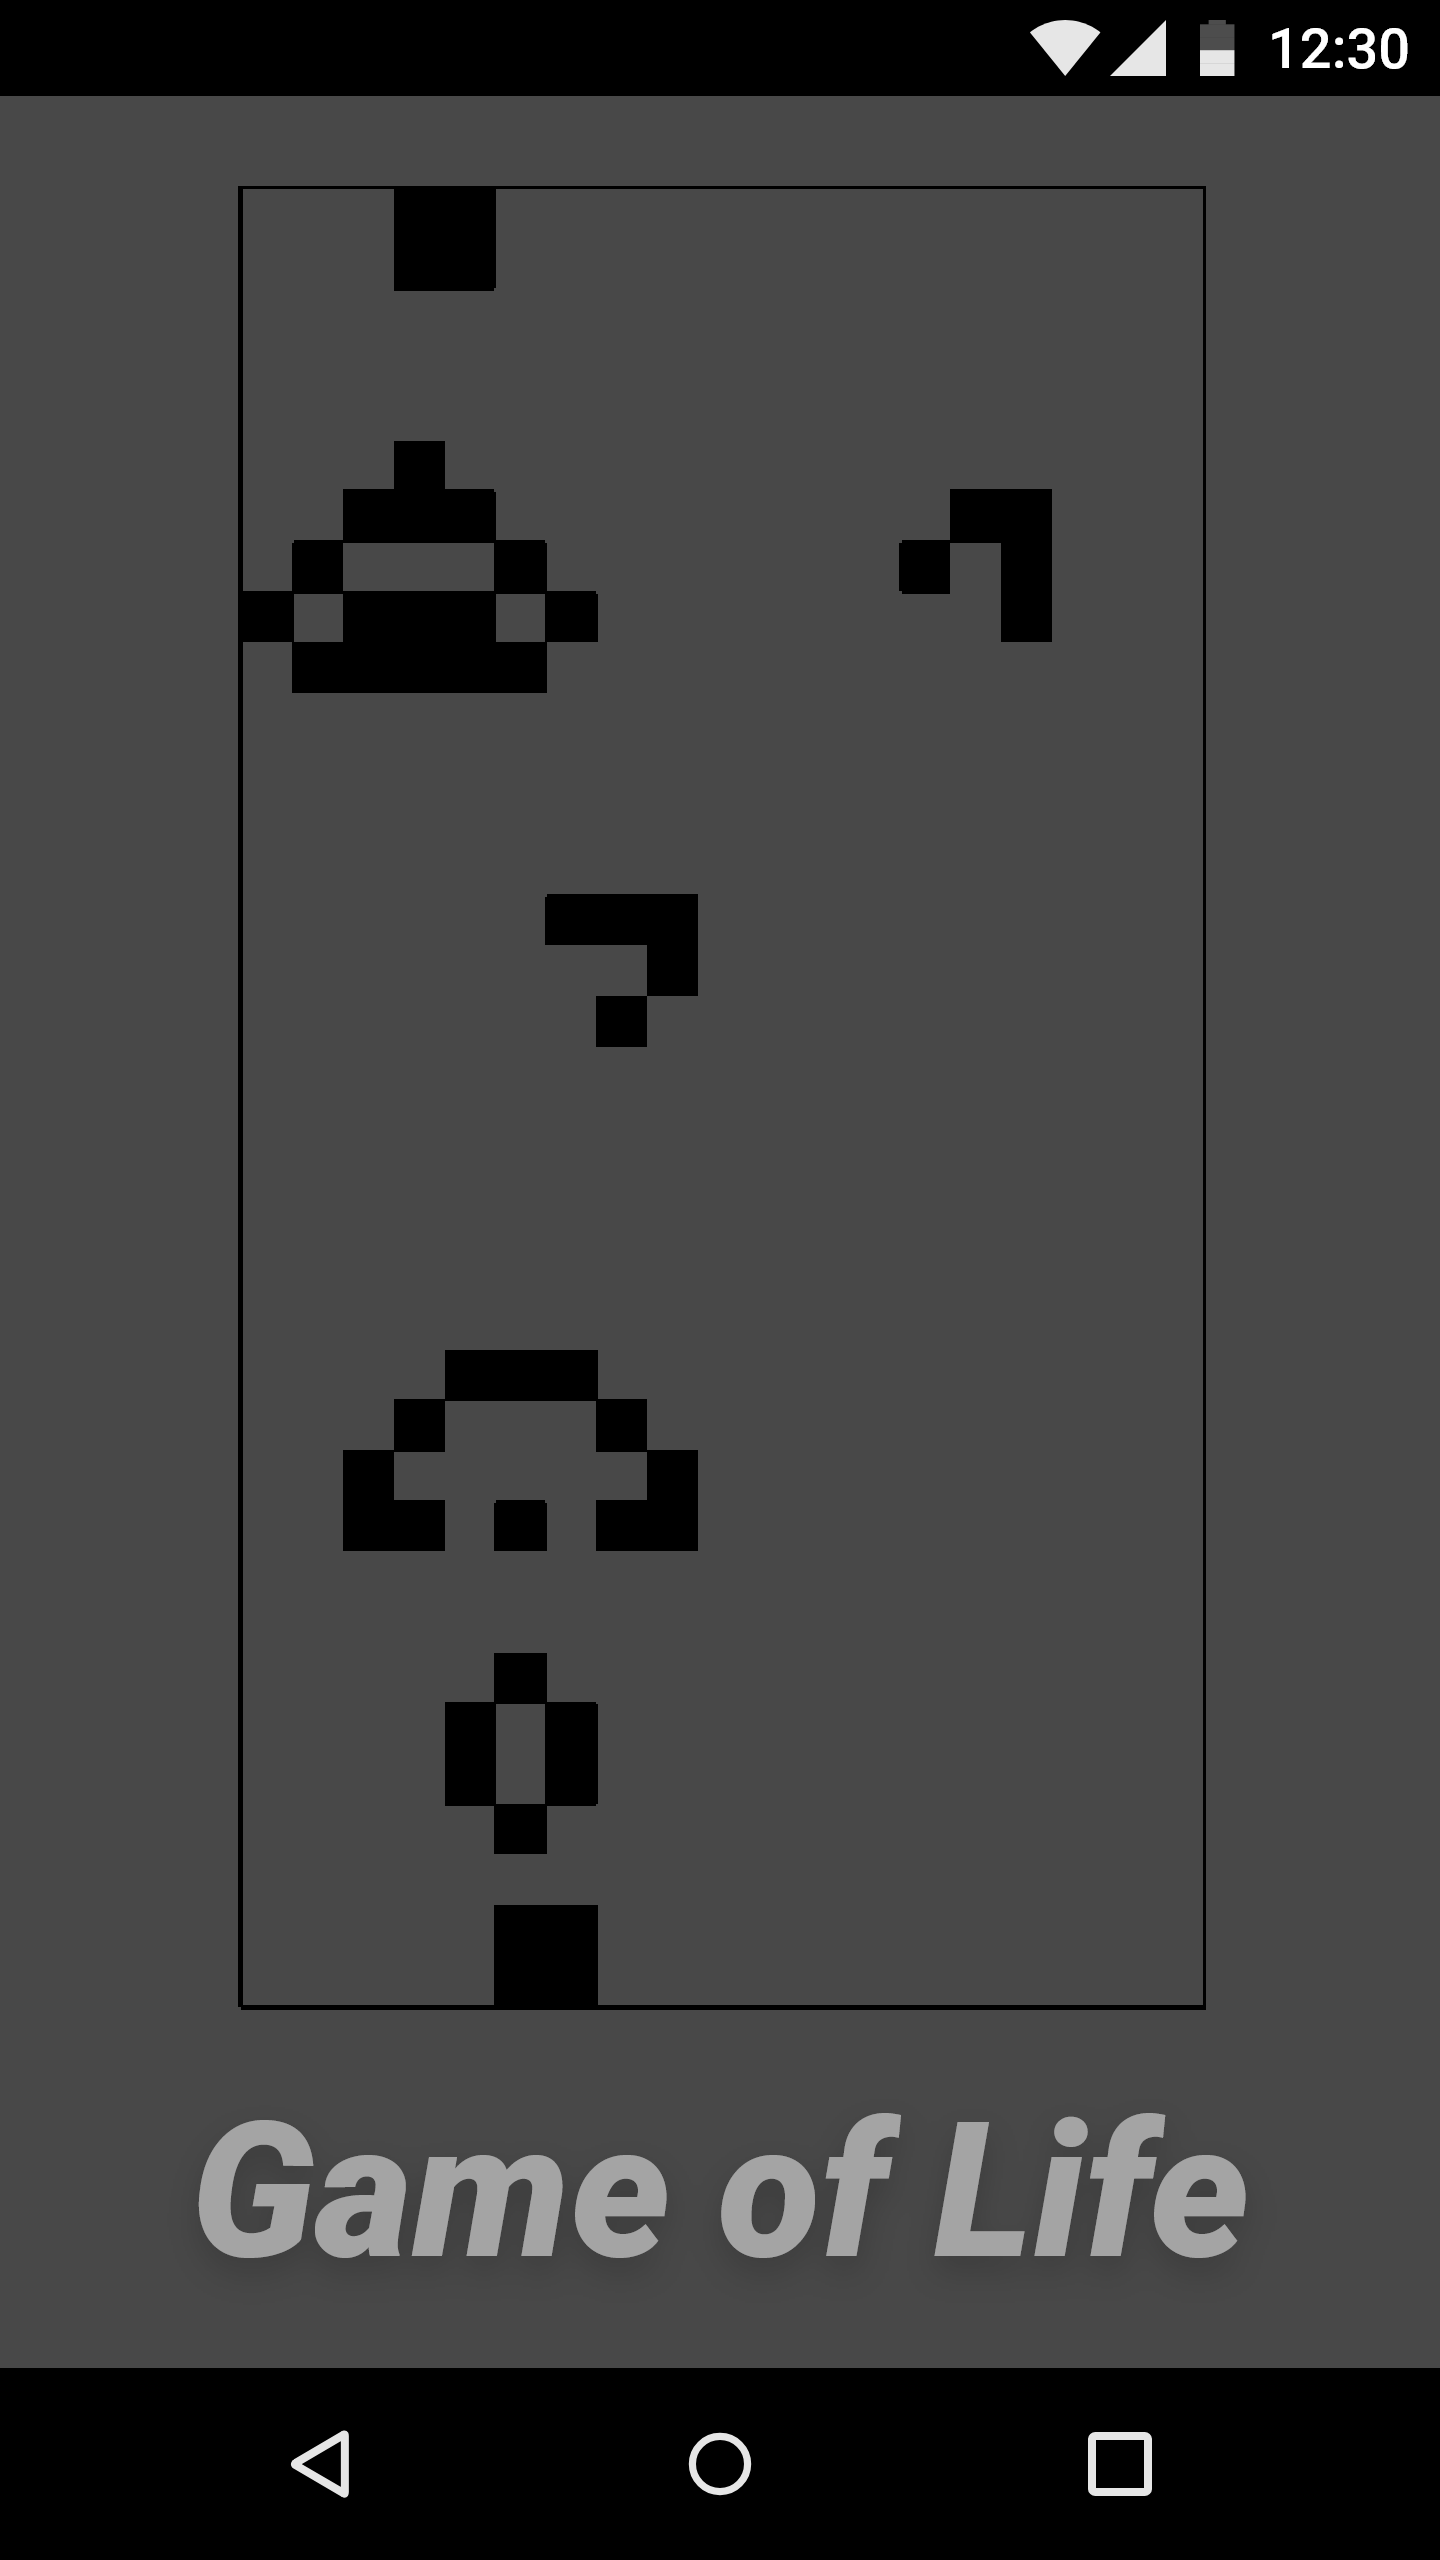
\includegraphics[width=0.33\textwidth]{Images/ui_splash.png}
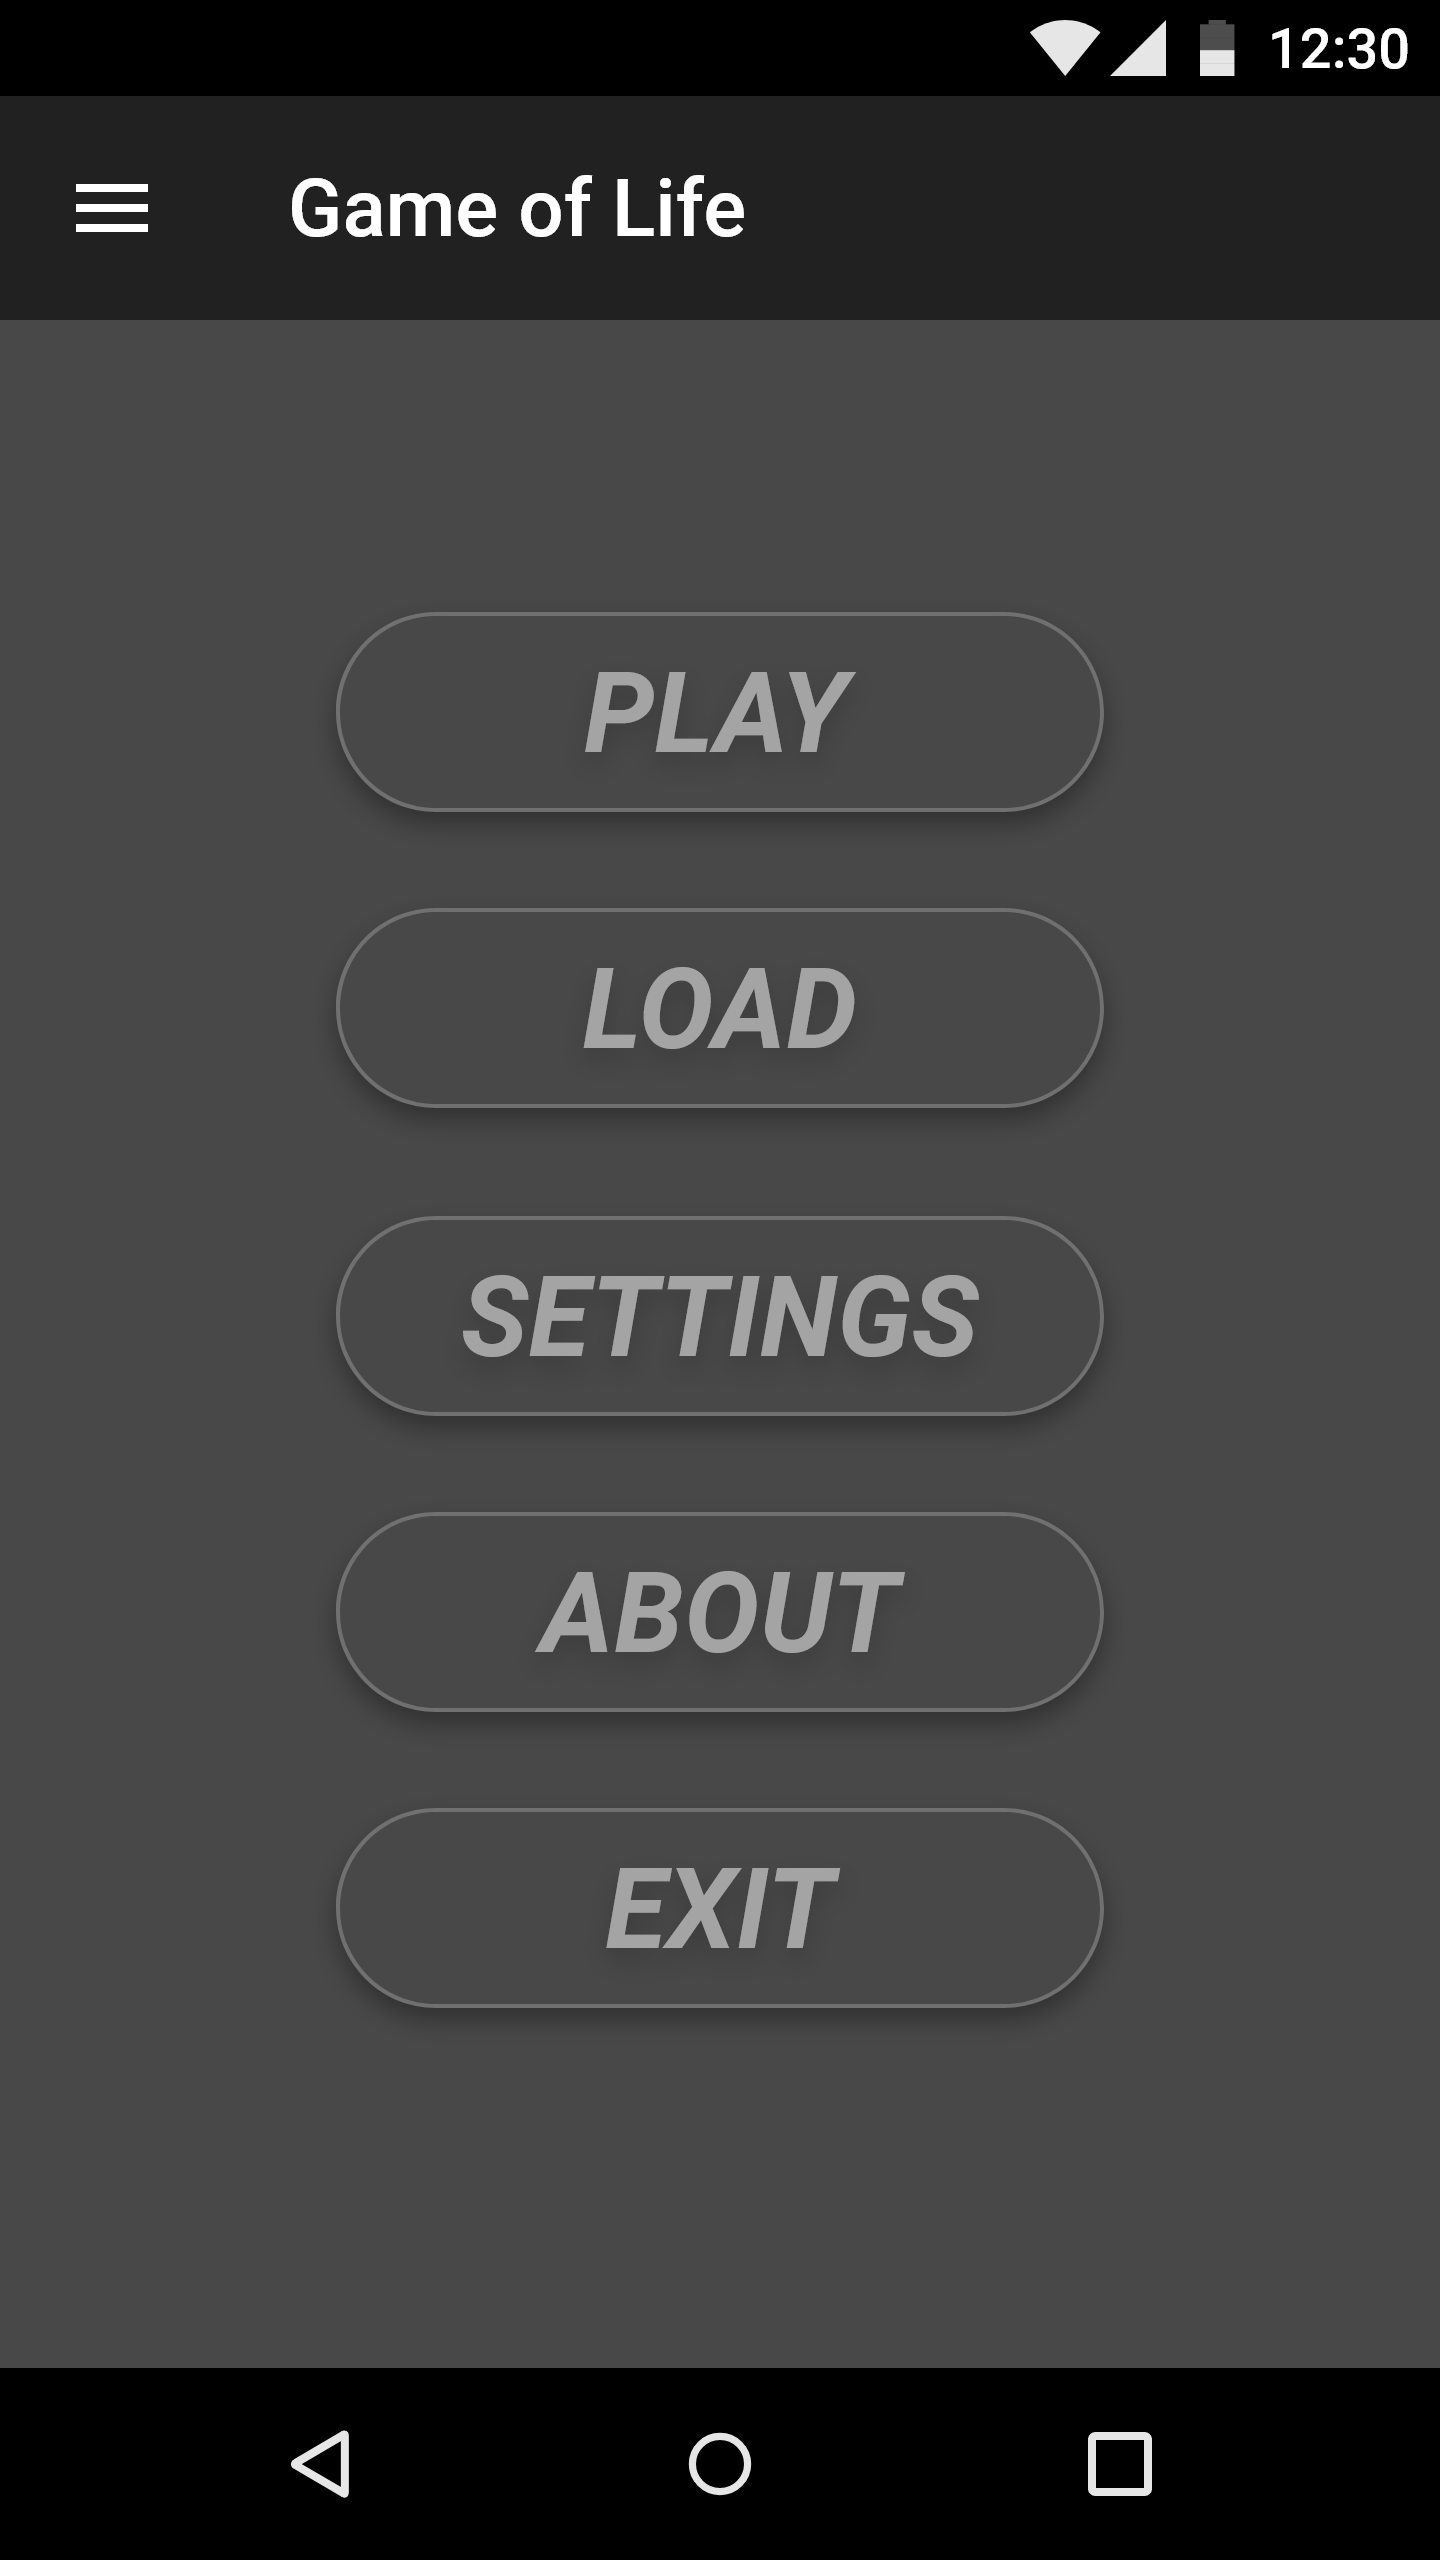
\includegraphics[width=0.33\textwidth]{Images/ui_main.png}
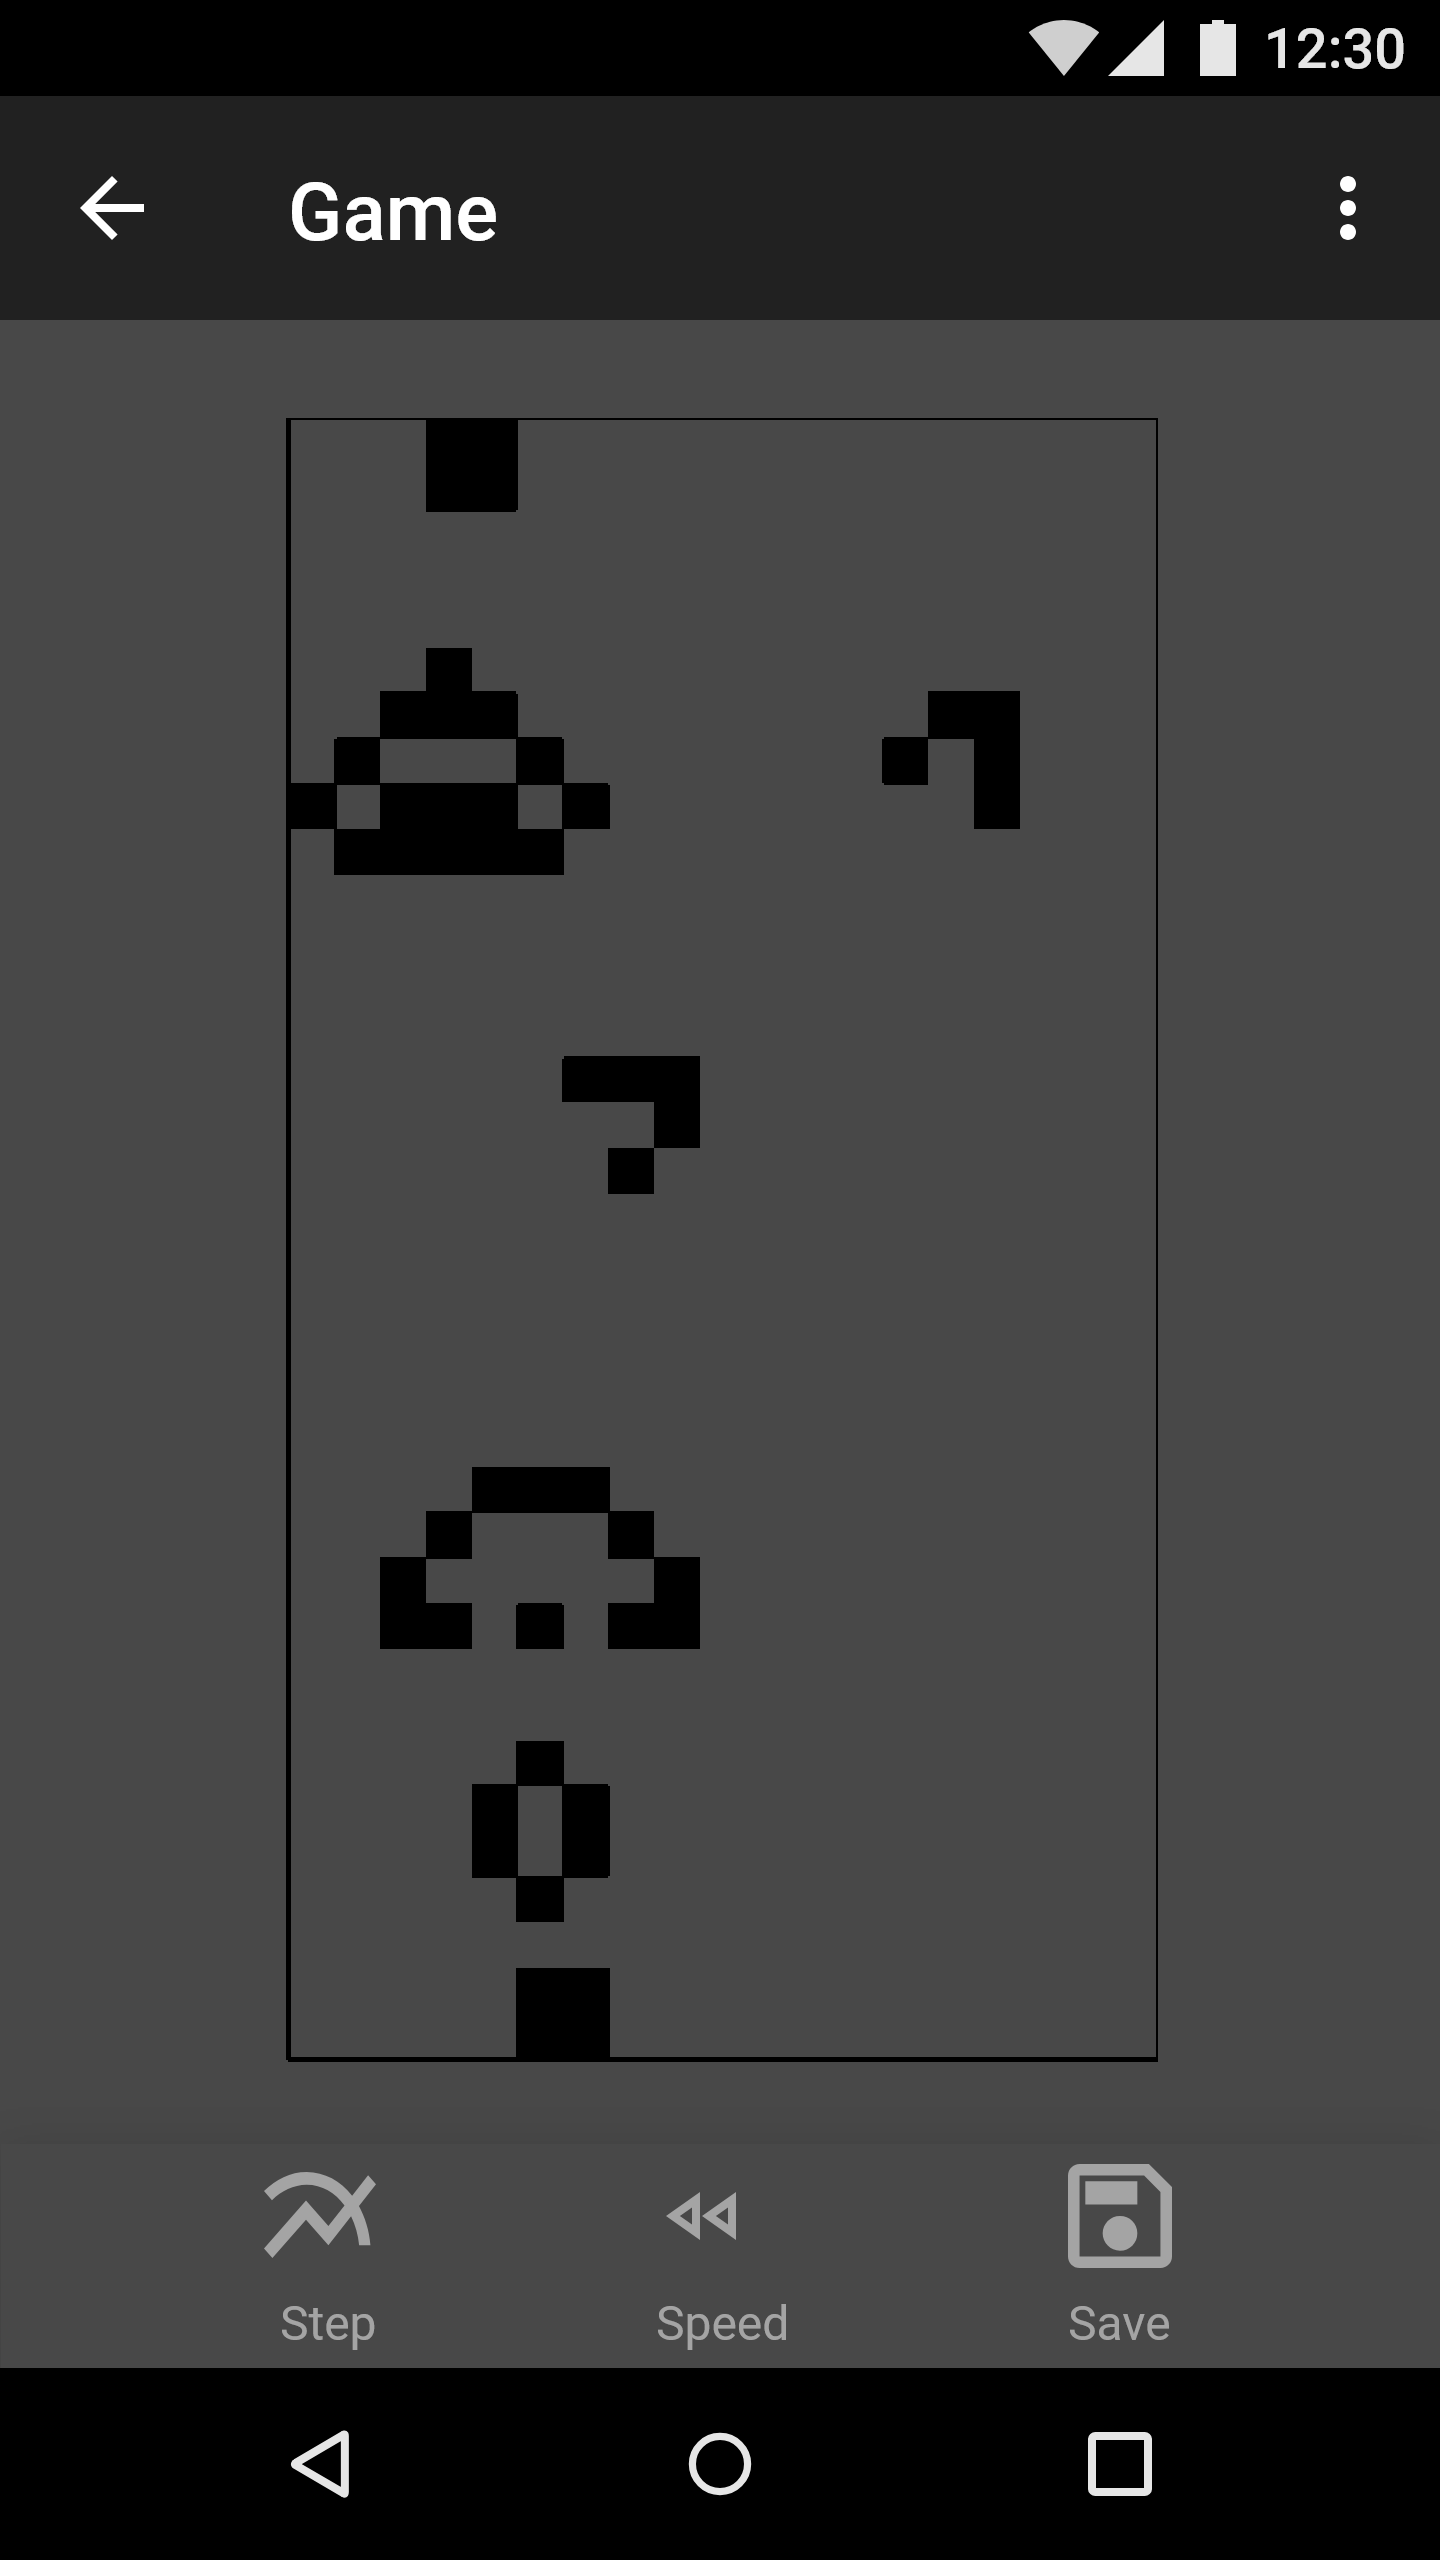
\includegraphics[width=0.33\textwidth]{Images/ui_game.png}
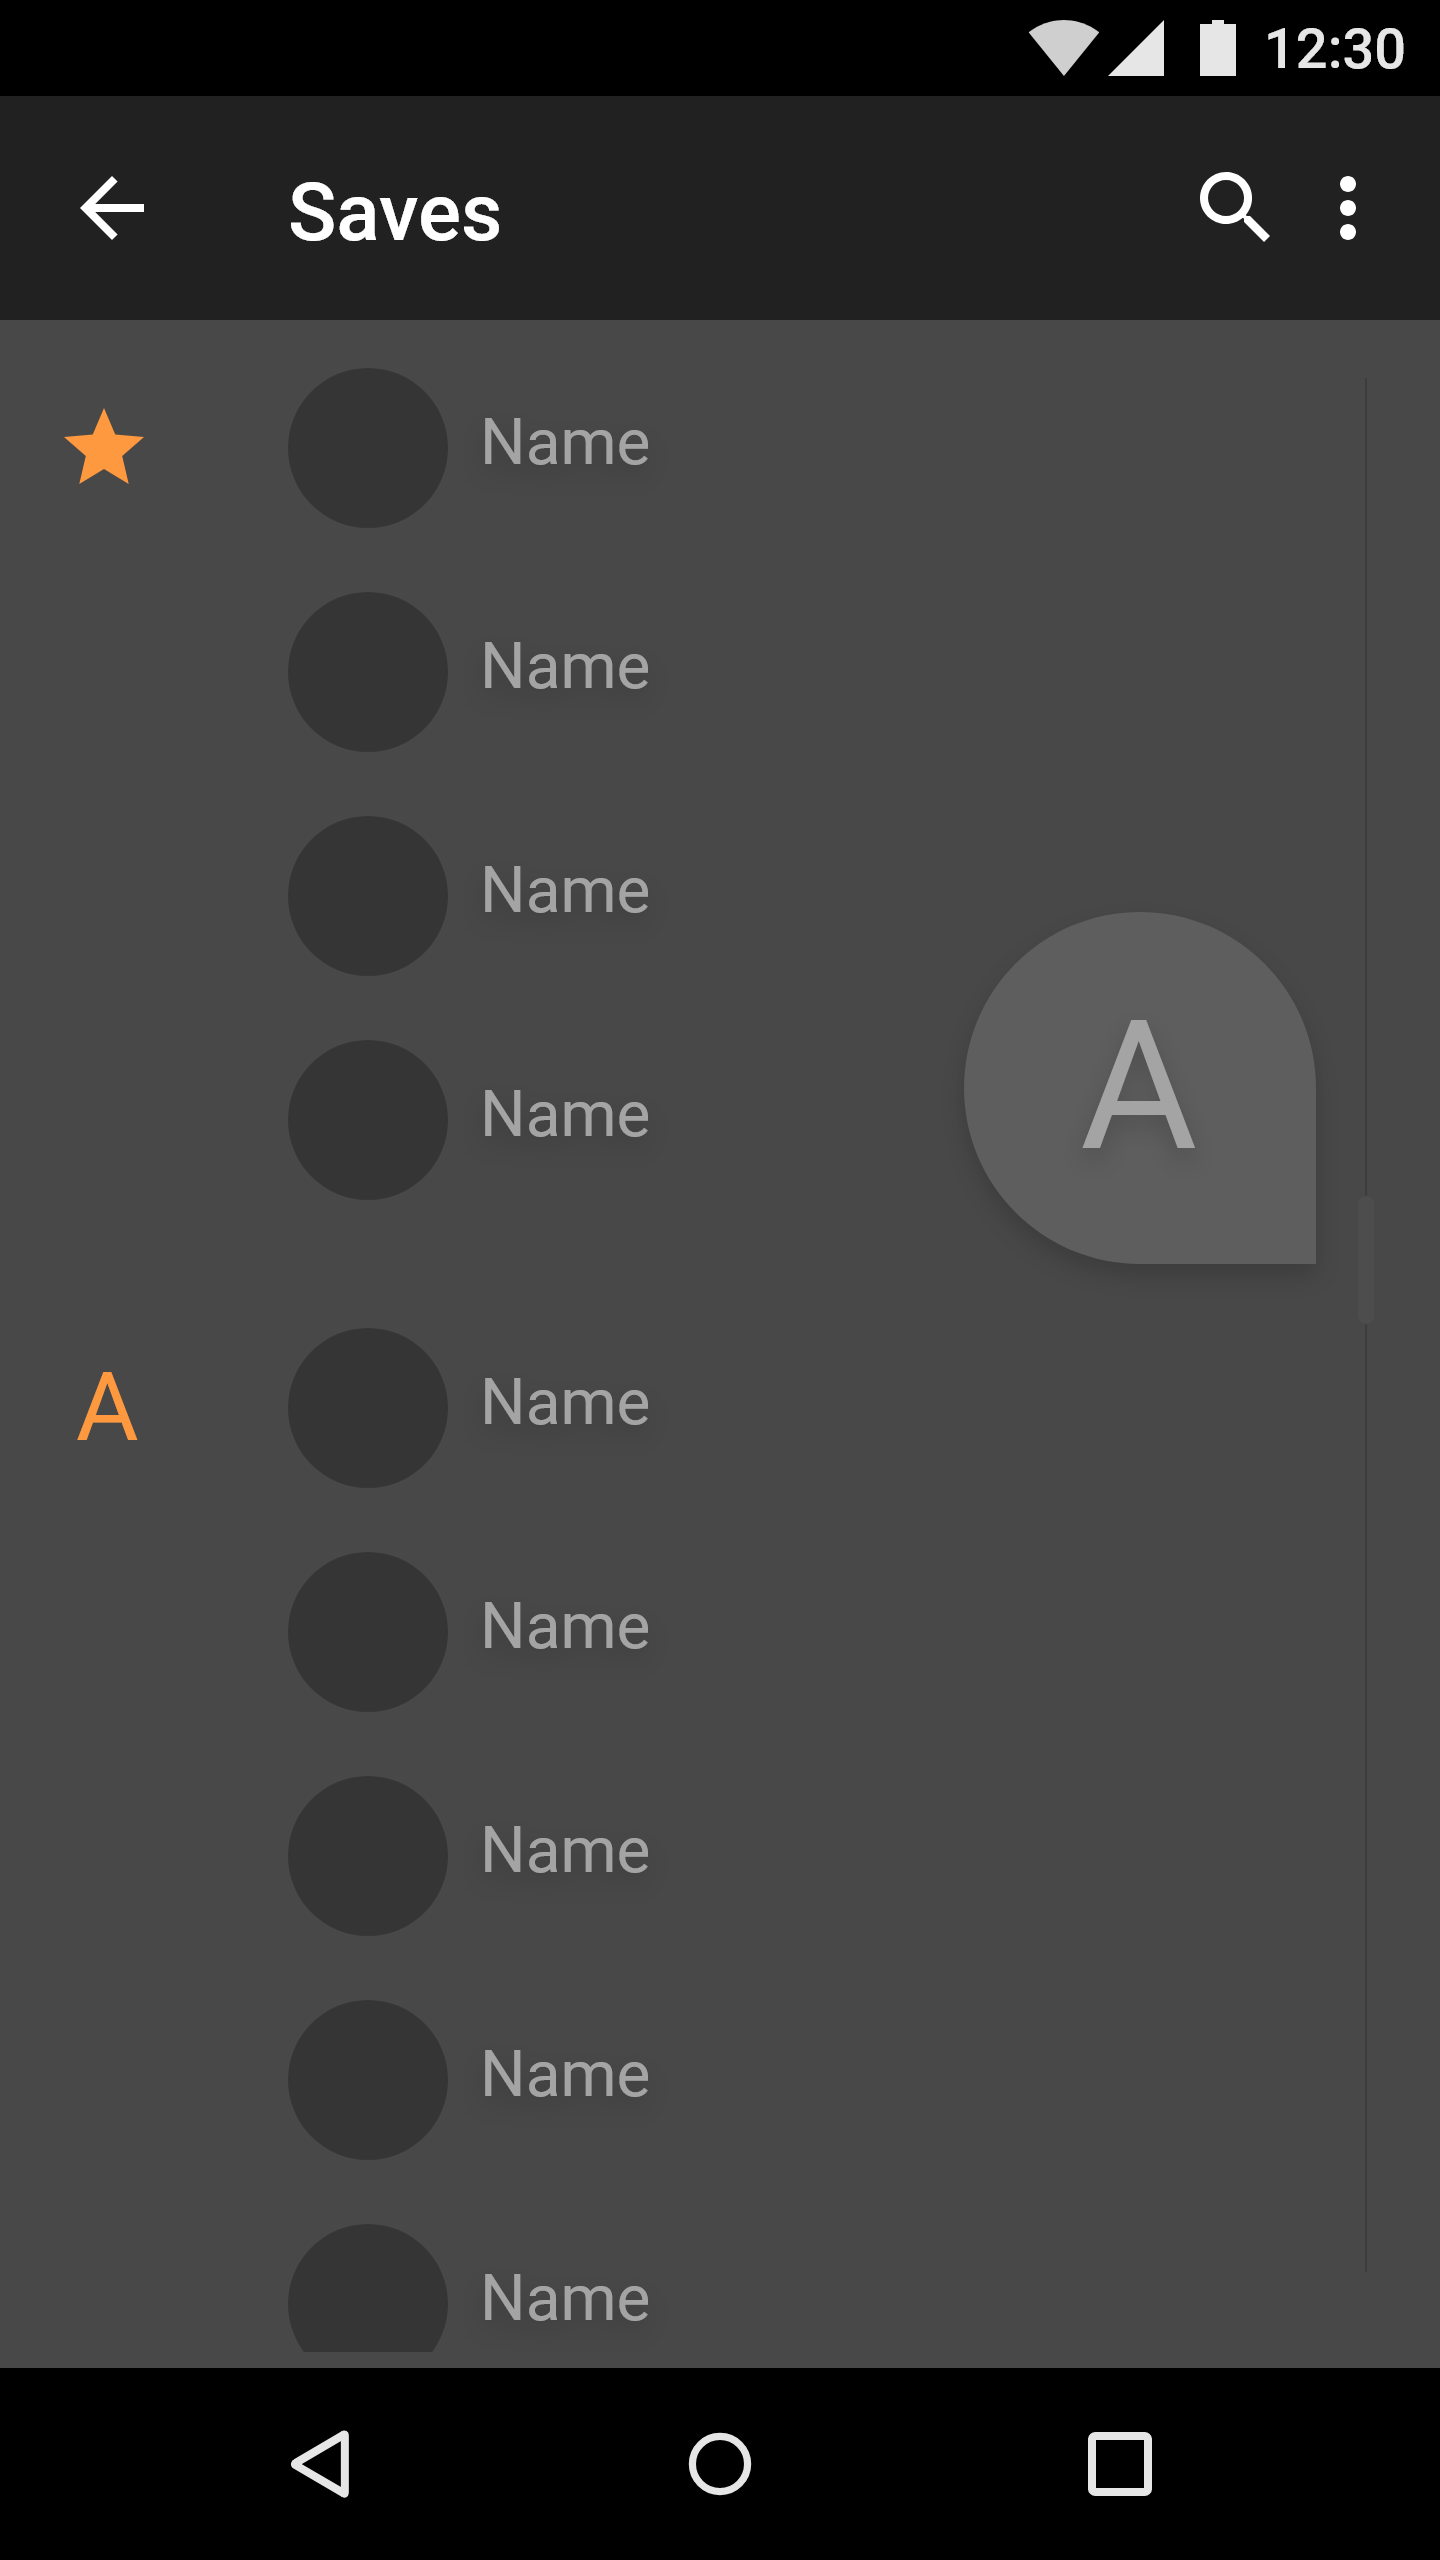
\includegraphics[width=0.33\textwidth]{Images/ui_saves.png}
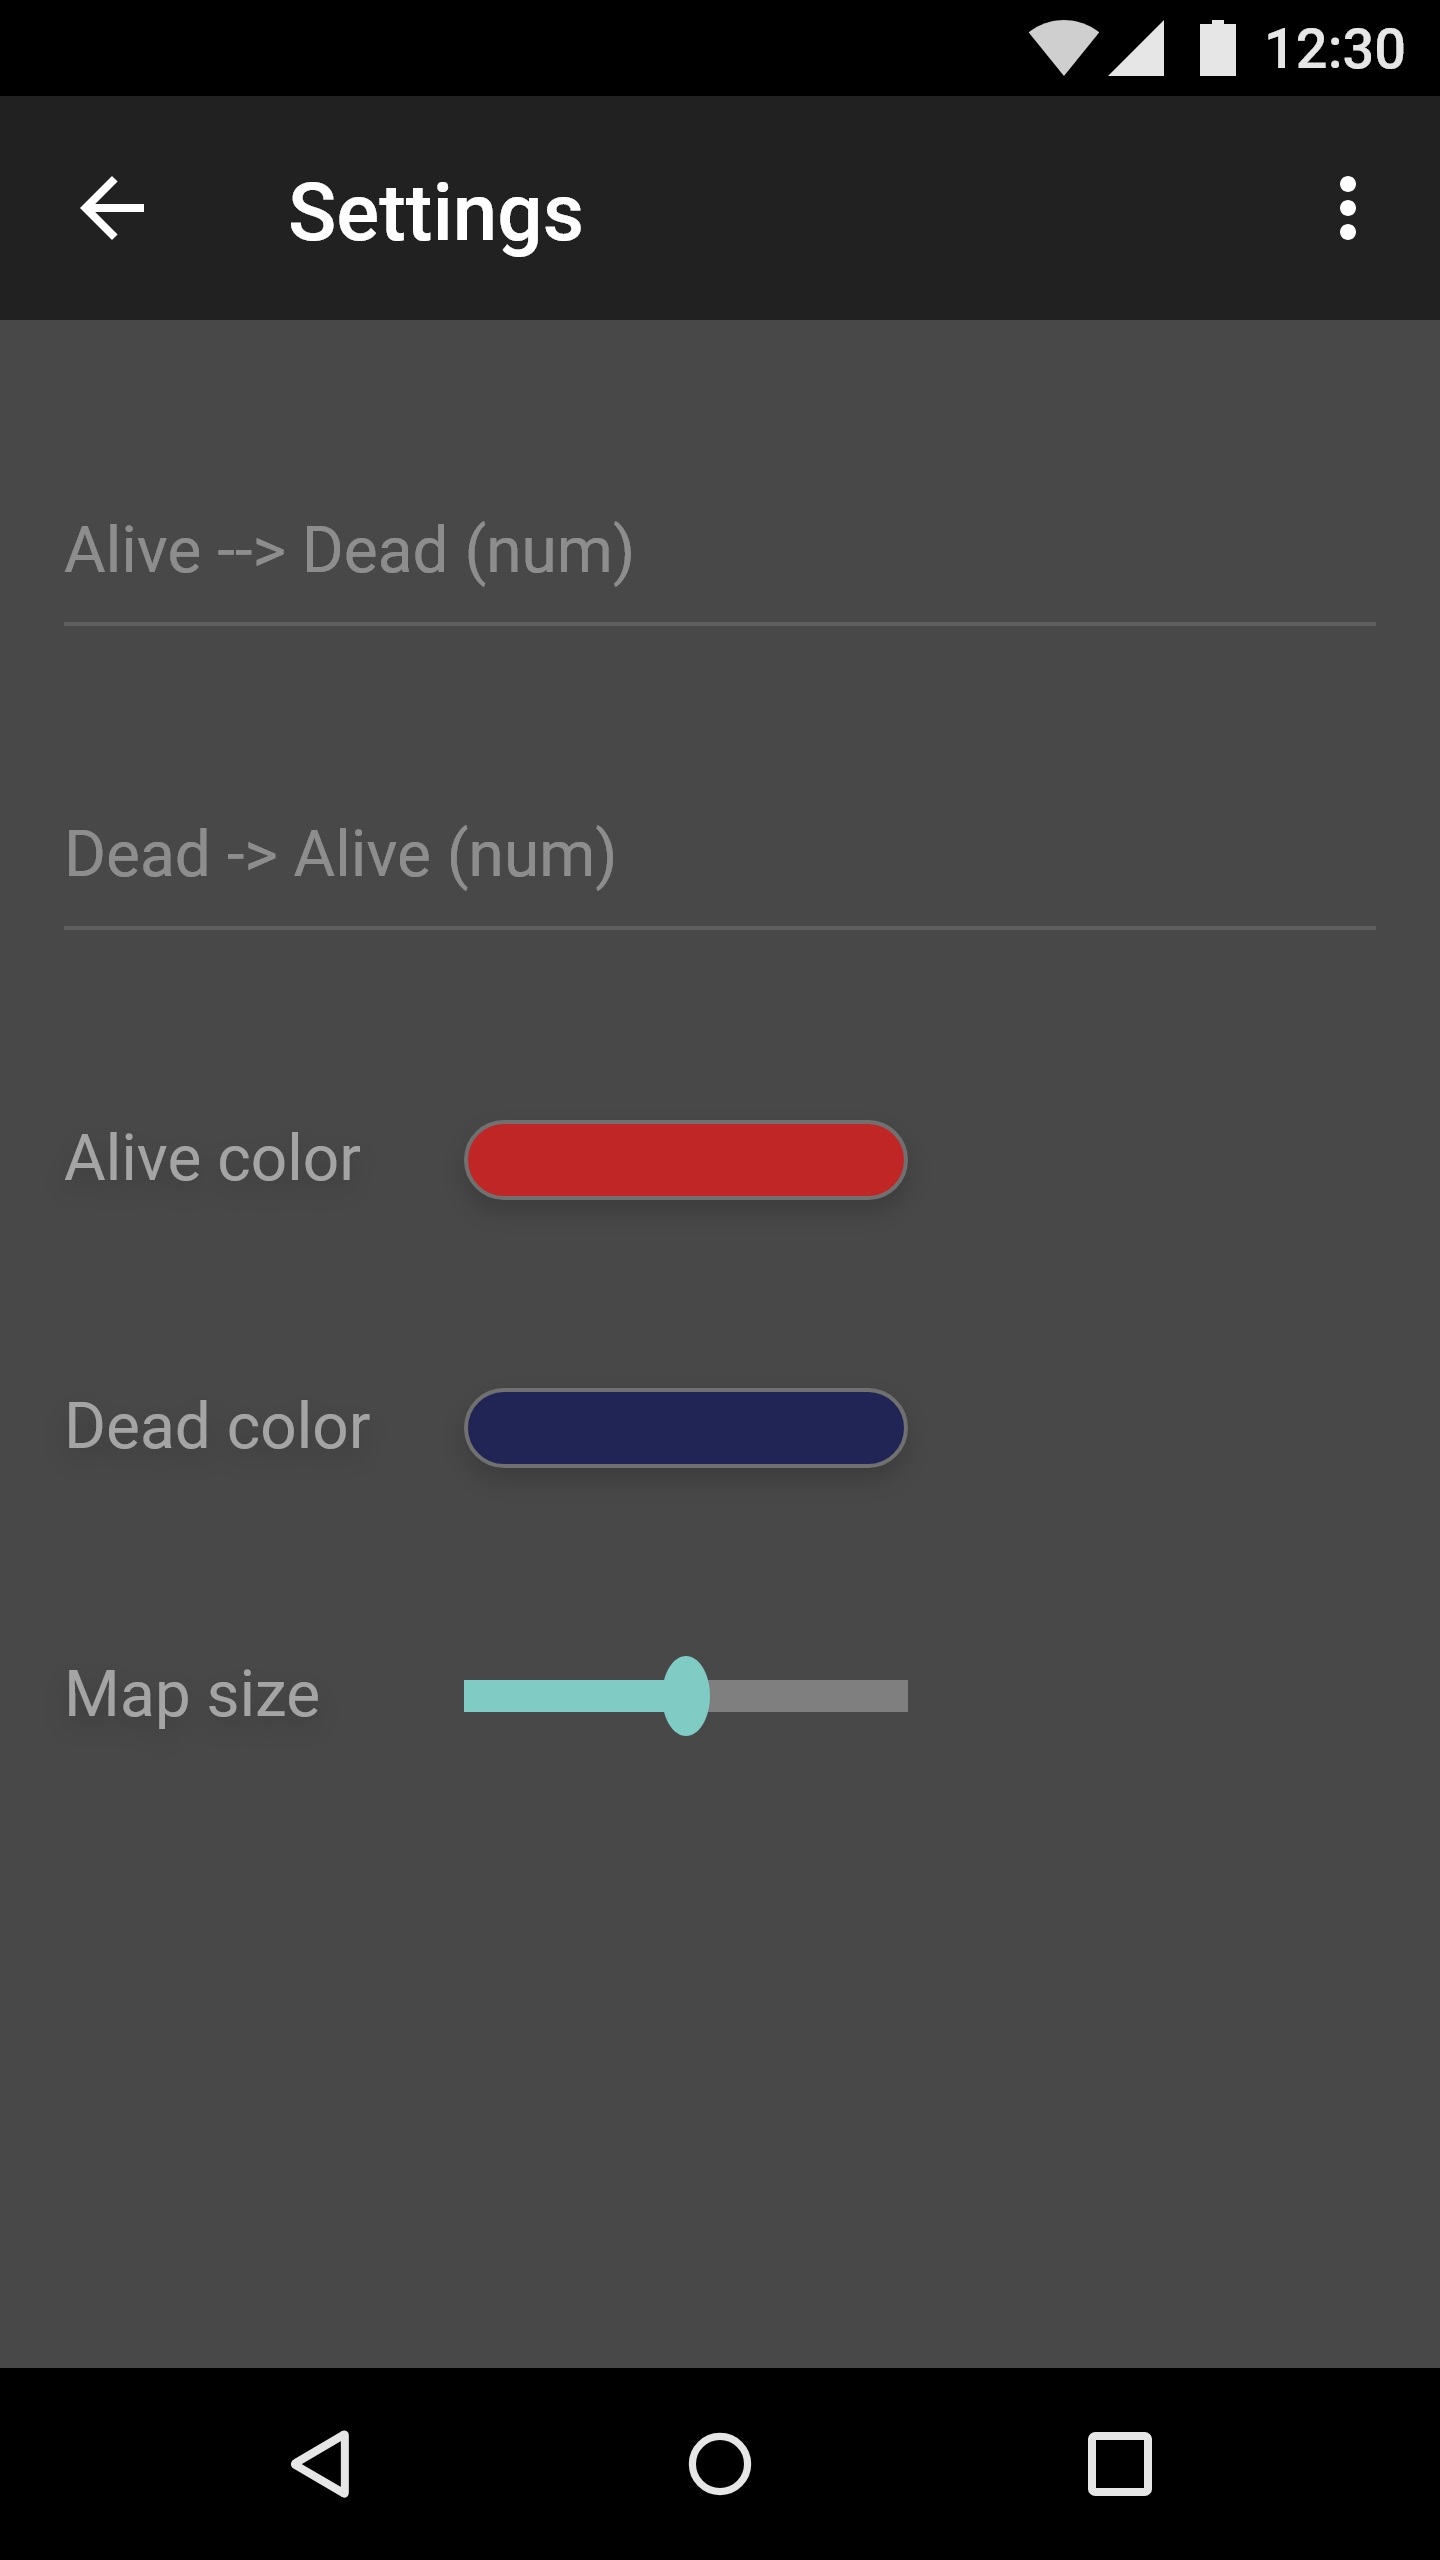
\includegraphics[width=0.33\textwidth]{Images/ui_settings.png}
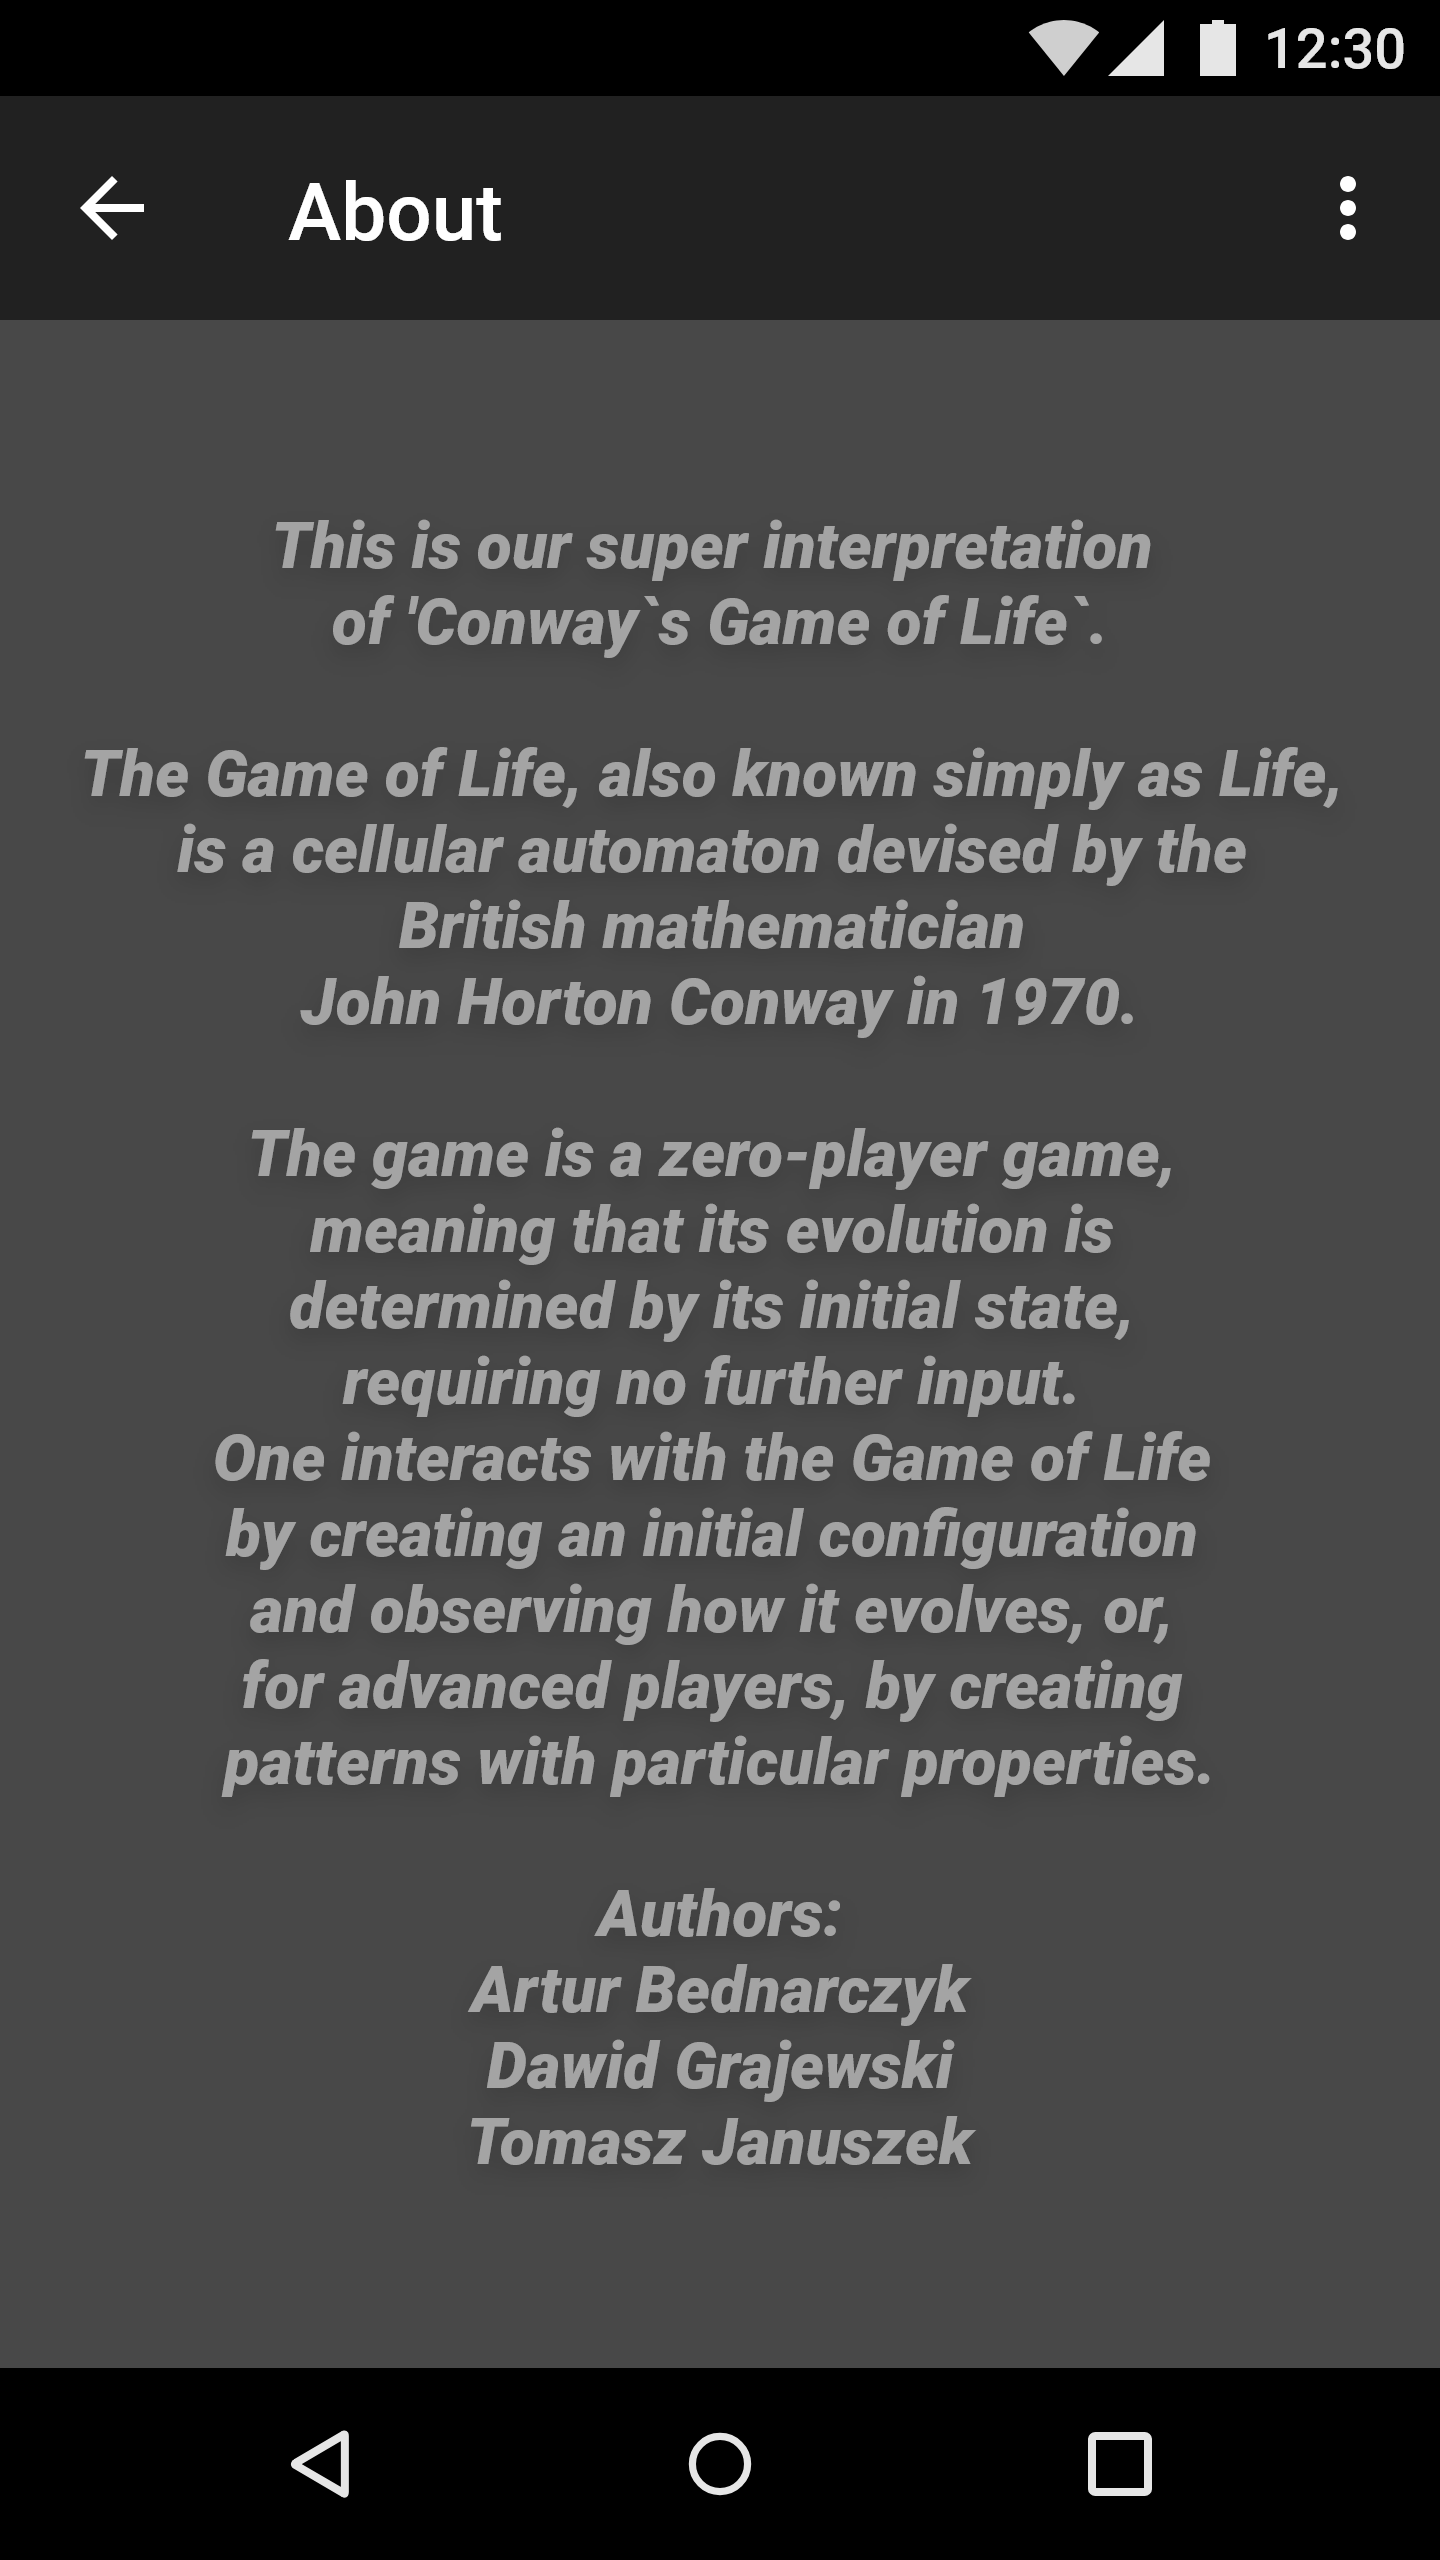
\includegraphics[width=0.33\textwidth]{Images/ui_about.png}
\section{Algorytmy}
\subsection{Aktualizacja gry}
Z każdym kolejnym krokiem krokiem aktualizowane są wszystkie komórki.
\begin{lstlisting}[language=Kotlin]
for (x in 0..(gameBoardSize - 1)) {
    for (y in 0..(gameBoardSize - 1)) {
        updateCellLife(x, y)
    }
}
\end{lstlisting}
Przy aktualizacji sprawdzany jest stan komórki, w zależności od którego sprawdzane są odpowiednie zasady, które są porównywane z stanem sąsiadów komórki.
\begin{lstlisting}[language=Kotlin]
if (gameBoard[x][y] == 1) {
    if (gameRules.neighboursToDie.contains(cellNeighbours)) {
        conwayTransitionGameBoard[x][y] = 0
    }
} else {
    if (gameRules.neighboursToBorn.contains(cellNeighbours)) {
        conwayTransitionGameBoard[x][y] = 1
    }
}
\end{lstlisting}
Gdzie stan sąsiadów, to liczba żywych komórek w otoczeniu sprawdzanej:
\begin{lstlisting}[language=Kotlin]
if (x > 0 && gameBoard[x - 1][y] == 1) {
    liveNeighbouringCellsCounter += 1
}
if (x < (gameBoardSize - 1) && gameBoard[x + 1][y] == 1) {
    liveNeighbouringCellsCounter += 1
}
if (y > 0 && gameBoard[x][y - 1] == 1) {
    liveNeighbouringCellsCounter += 1
}
if (y < (gameBoardSize - 1) && gameBoard[x][y + 1] == 1) {
    liveNeighbouringCellsCounter += 1
}
if (x > 0 && y > 0 && gameBoard[x - 1][y - 1] == 1) {
    liveNeighbouringCellsCounter += 1
}
if (x > 0 && y < (gameBoardSize - 1) && gameBoard[x - 1][y + 1] == 1) {
    liveNeighbouringCellsCounter += 1
}
if (x < (gameBoardSize - 1) && y > 0 && gameBoard[x + 1][y - 1] == 1) {
    liveNeighbouringCellsCounter += 1
}
if (x < (gameBoardSize - 1) && y < (gameBoardSize - 1) && gameBoard[x + 1][y + 1] == 1) {
    liveNeighbouringCellsCounter += 1
}
\end{lstlisting}
\section{Narzędzia}
\subsection{Kontrola wersji}
Do zarządzania kodem i wersjami projektu wykorzystujemy narzędzie Git. Korzystamy z platformy GitHub jako repozytorium dostępnego online. Dobór narzędzi służących do korzystania z repozytorium to sprawa indywidualna każdego członka zespołu, ponieważ nie ma ona wpływu na sam projekt.

\subsection{Zarzadzanie zespołem}
Trello - Kanban Board - to tutaj rozpisujemy zadania i przydzielamy je sobie, określamy również terminy i planujemy.\\

Przy współpracy, aby dane zmiany zostały wprowadzone muszą zostać akceptowane przez innego członka zespołu.
\subsection{Środowisko}
Android Studio - Kotlin \\
\section{Aplikacja}
\subsection{Architektura}
Aplikacja została utworzona zgodnie z architekturą MVVM (Model-View-ViewModel)\\
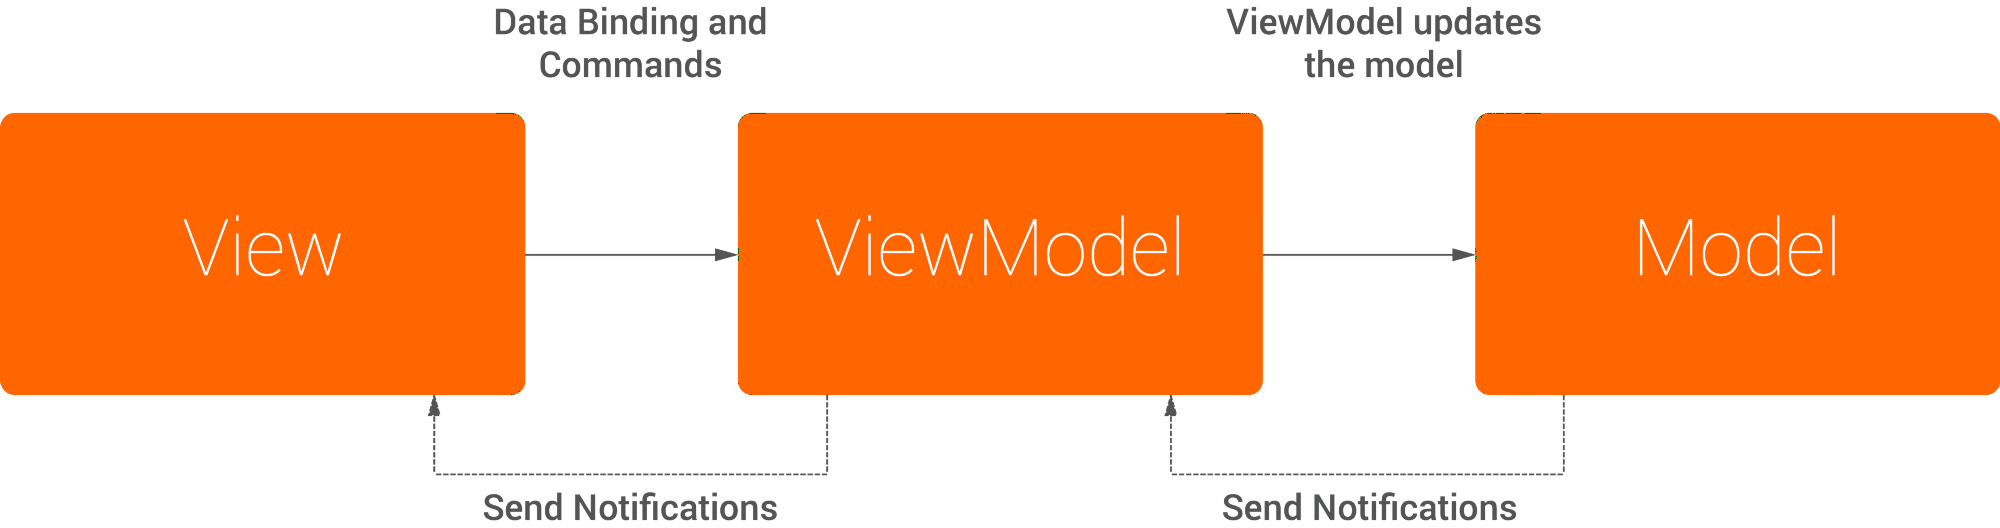
\includegraphics[width=1\textwidth]{Images/mvvm.png}\\
Dzięki ,,Data binding`` dane przechowywane przez model są automatycznie odświeżanie w widoku. View, jako warstwa widoku zawiera interfejs użytkownika oraz odpowiada za interakcję z użytkownikiem. Viewmodel jest warstwą modelu widoku, która udostępnia dane i odpowiada za wymianę informacji z modelem. Przechowuje również referencje do modelu. Model zawiera logikę aplikacji.
\subsection{Struktury danych}
Reguły gry w życie przechowujemy jako ciąg liczb określających liczbę sąsiadów, oddzielany średnikiem. Przykład: \\
''0;1;2;3;'' \\
Kolory są w formacie ARGB. \\
Zapis stanu do pliku w formacie JSON, przykład:\\ 
\begin{lstlisting}[language=json]
{ 
	x: 3,
	y: 3,
	birth: "1;2;3;",
	death: "4;5;",
	aliveColor: -1,
	deadColor: -16777216,
	gameState: 	[1,0,0,
			1,0,1,
			1,0,1,]
}
\end{lstlisting}
\subsection{Schemat graficzny struktury systemu}
\subsection{Podział na pliki}
\begin{multicols}{2}
\scalebox{0.7}[0.7]{
			\begin{forest}
				for tree={font=\sffamily, grow'=0,
    folder indent=.3em, folder icons}
    	[Main
    	    [.model
				[.algorithm
					[ConwayAlgorithm, is file]
					[IConwayAlgorithm. is file]				
				]
				[.bitmap
					[BitmapGenerator, is file]				
					[IBitmapGenerator, is file]
				]
				[.dto
					[ActivityStartModel, is file]				
				]
				[.event
					[SingleLiveEvent, is file]				
				]
				[.pref
					[.serializer
						[GameRulesSerializer, is file]
						[IGameRulesSerializer, is file]		
					]
					[IColorPref, is file]
					[IGameRulesPref, is file]
					[SharedPrefAccess, is file]
				]
				[.setting
					[GameColors, is file]
					[GameRules, is file]
					[ViewProperties, is file]
				]
				[.simulation
					[ILooper, is file]
					[LooperImp, is file]
					[SpeedModel, is file]
				]    	    
    	    ]
    	 ]
    	 \end{forest}
		\begin{forest}
				for tree={font=\sffamily, grow'=0,
    folder indent=.3em, folder icons}
    [.Main
     		[.util
				[Extensions, is file]    	    
    	    ]
    	    [.view.acivity
    	    	[.contract
					  [BackActivity, is file]  	    	
    	    	]
				[AboutActivity, is file]    	    
				[GameActivity, is file]
				[LoadActivity, is file]
				[MenuActivity, is file]
				[SettingsActivity, is file]
				[SplashActivity, is file]
    	    ]
    	    [.viewmodel
				[GameViewModel, is file]
				[LoadViewModel, is file]
				[MenuViewModel, is file]
				[SettingsViewModel, is file]    	    	
    	    ]
    	    [GameOfLifeApplication, is file]
       	]
			\end{forest}
			}

		\end{multicols}
\subsection{Biblioteki}
W projekcie zostały wykorzystane następujące biblioteki:
\begin{itemize}
\item Lifecycle library - zarządzanie aktywnościami i cyklem życia
\item Koin - wstrzykiwanie zależności
\item Dexter - zarządzanie uprawnieniami
\item QuadFlask:colorpicker - wybieranie kolorów
\item Timber - logowanie
\end{itemize}
\subsection{Testowanie}
Aplikacja jest testowana testami jednostkowymi oraz manualnie. Jednostkowo została przetestowana klasa ,,GameRulesSerializer``
\end{document}